%!TEX root = ../../main.tex
\chapter{性能評価・考察}
本研究の評価として,tap認識の精度と調性制約の評価実験を行った.
%--------%---------%---------%--------%---------%---------
\section{実験内容}
20代から50代の男女12人に本システムを実際に体験してもらい,評価用紙の質問に答えてもらう.
%インタフェースの操作に慣れてくると後に操作した手法の評価に影響を受けてしまうおそれがあるため,条件を平等にするため被験者の半分には提案手法のあと比較手法,残り半分には比較手法のあと提案手法の順序で実験をしてもらった.
減衰音を出力するtap動作の認識手法については,第3章で説明した提案手法に対し,RealSense SDKで用意されたデフォルトの認識との比較を行った.調性制約の生成手法については,第5章で説明した提案手法に対し,単純に背景楽曲のコードの構成音を調性制約として用いる手法との比較を行った.ただし,提案手法と比較手法の順序が固定されていると被験者による操作習熟の影響が生じるため,半分の6人は提案手法が先で比較手法が後,もう半分の6人は比較手法が先で提案手法が後になるように,実験を行った.
\subsection{tap評価実験}
第3章で説明したtap認識の提案手法とRealSense SDK で用意されたデフォルトのtap認識の2つの方法で,背景楽曲の拍を表す円に合わせてtapをしてもらい,各実験の後図\ref{img:eval1}の二つの質問に答えてもらった.
\begin{figure}[ht]
	\begin{center}
		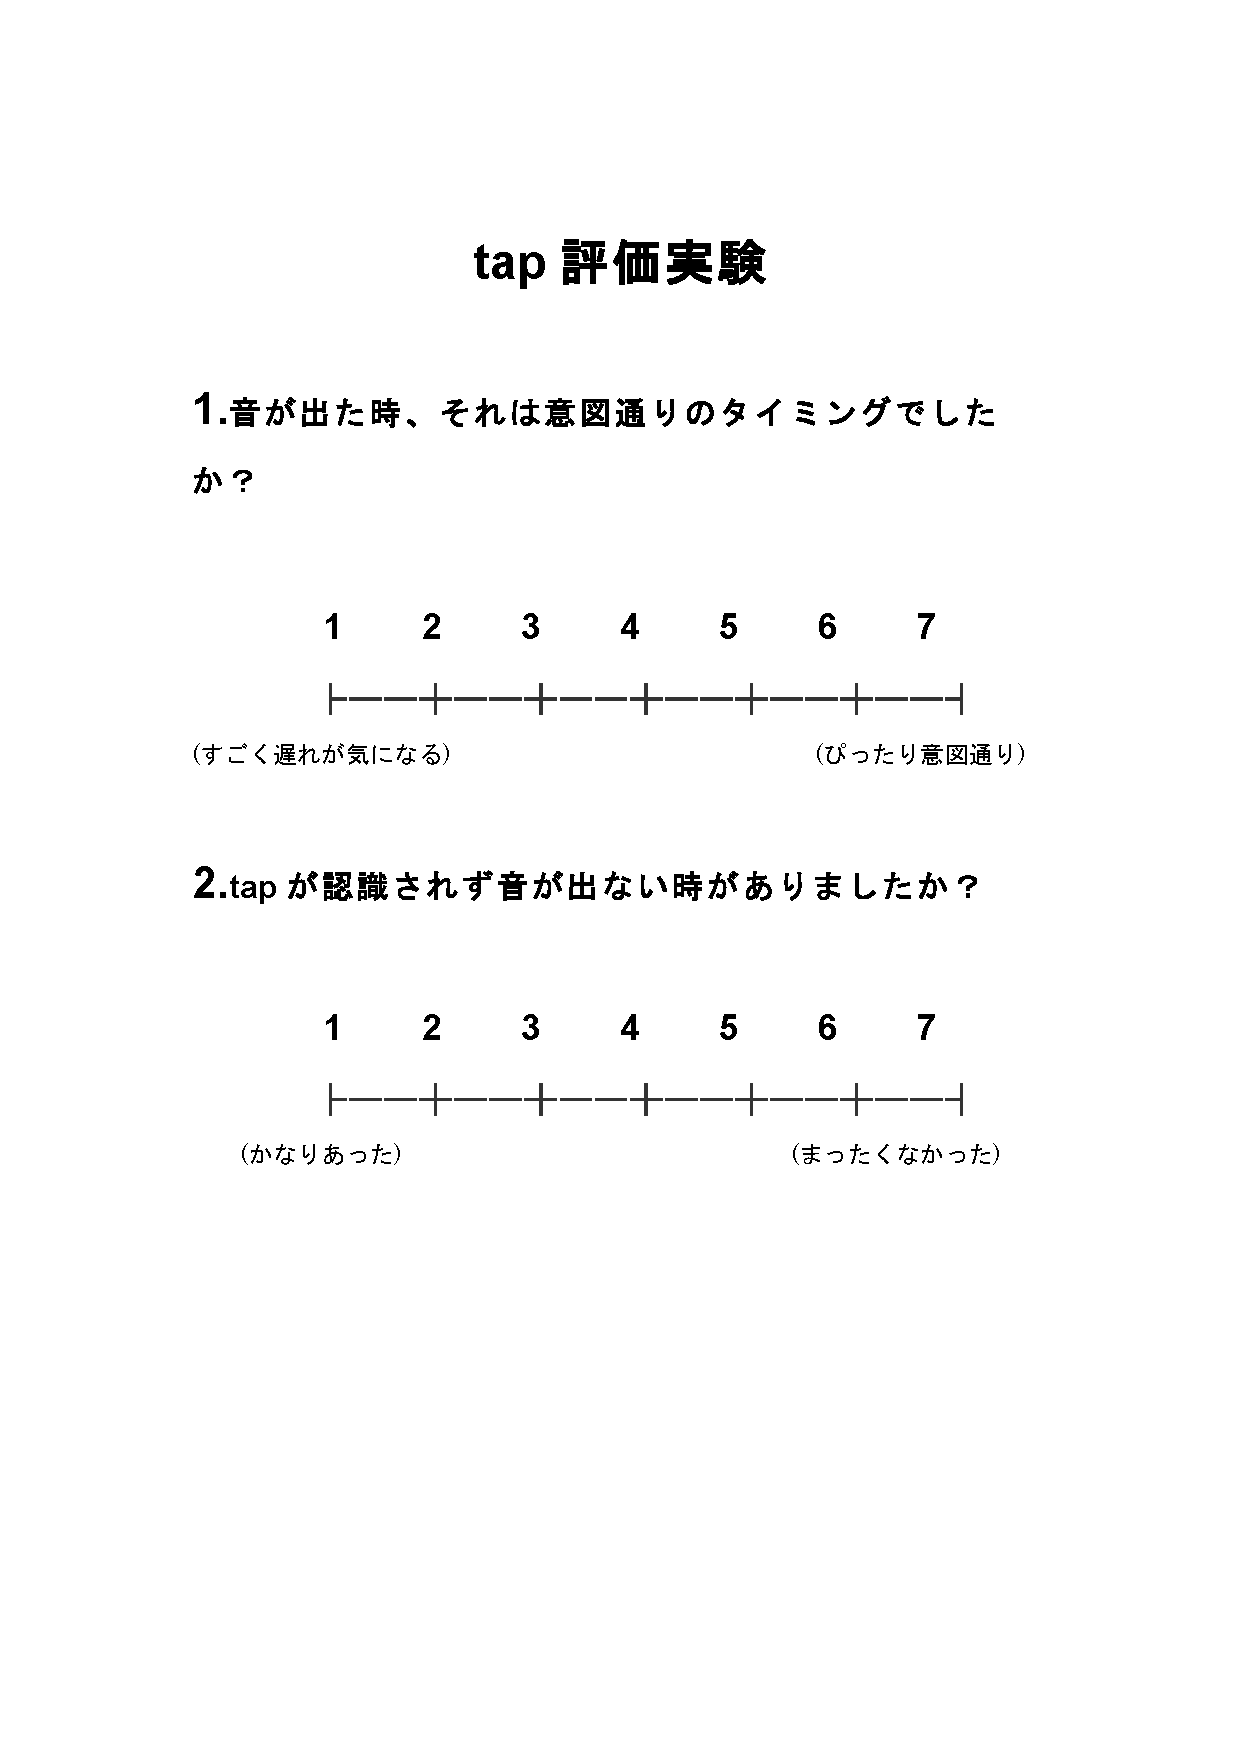
\includegraphics[width=1.0\linewidth]{part/06.Evaluation/tap.pdf}
		\caption{tap評価用紙}
		\label{img:eval1} 
	\end{center}
\end{figure}

\subsection{調性制約評価実験}
コードの構成音のみを周波数列にもつ調性制約と,Songleのデータから統計的に生成した調性制約で演奏してもらい,各演奏の後図\ref{img:eval2}の2つの質問に答えてもらった.
\begin{figure}[ht]
	\begin{center}
		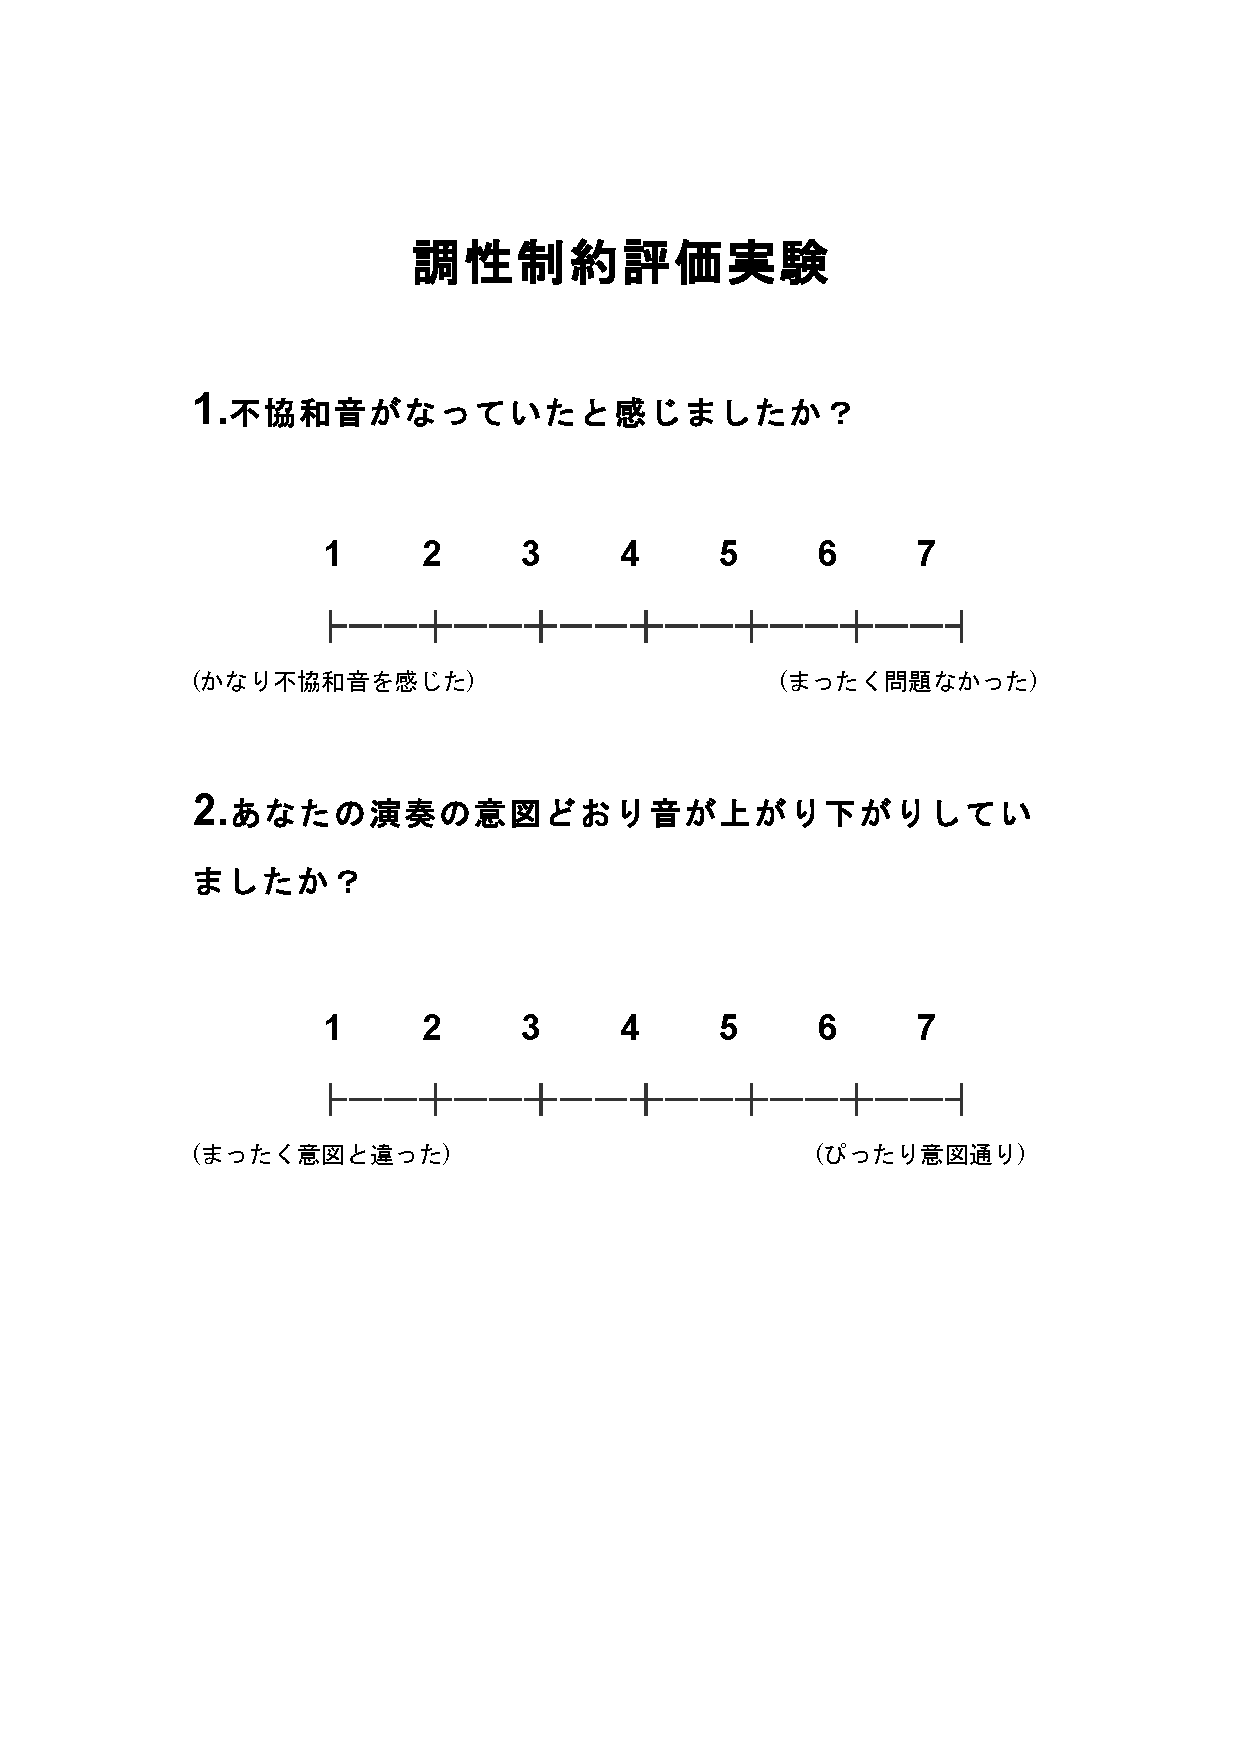
\includegraphics[width=1.0\linewidth]{part/06.Evaluation/tonality.pdf}
		\caption{調性制約評価用紙}
		\label{img:eval2}
	\end{center}
\end{figure}
\section{実験結果と考察}
tap評価実験の結果の平均を図\ref{img:result1}に示す.調性制約評価実験の結果の平均を図\ref{img:result2}に示す.図\ref{img:result1}より,本研究で実装したtap認識の方がRealSense SDKのtap認識よりも高い評価を得ているので,実用的であると言える.図\ref{img:result2}より統計的に生成した調性制約は,コードの構成音のみを周波数列にもつ調性制約と比べ不協和音が含まれるが,わずかに意図通りの演奏がしやすいという評価を得た.これはコードの構成音にさらに音を追加したことで表現の幅が広がったためと思われる.不協和音が多いため,追加する音を決める閾値の調節または追加する手法の検討を今後の課題としたい.
\begin{figure}[ht]
	\begin{center}
		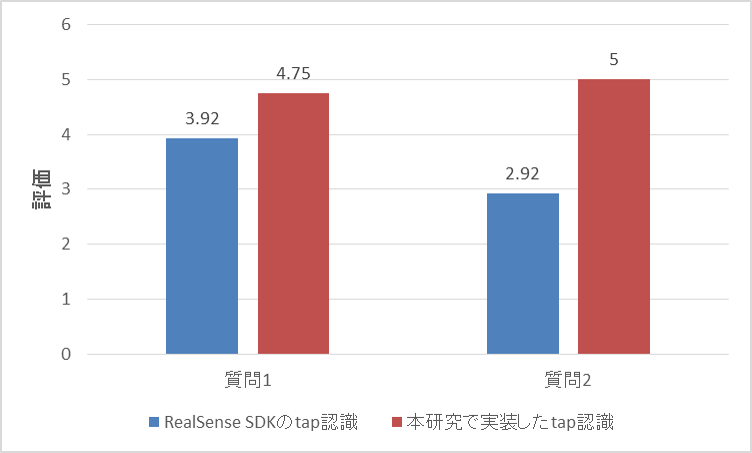
\includegraphics[width=1.0\linewidth]{part/06.Evaluation/evalresult1.png}
		\caption{tap評価実験結果}
		\label{img:result1} 
	\end{center}
\end{figure}
\begin{figure}[ht]
	\begin{center}
		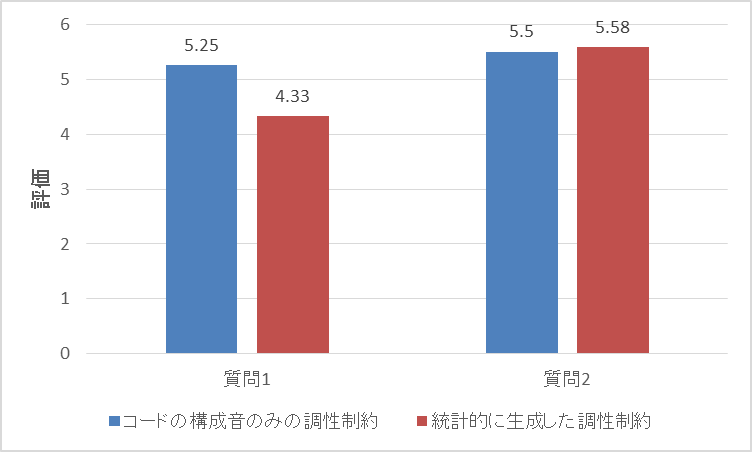
\includegraphics[width=1.0\linewidth]{part/06.Evaluation/evalresult2.png}
		\caption{調性制約評価実験結果}
		\label{img:result2} 
	\end{center}
\end{figure}